\documentclass[output=paper,colorlinks,citecolor=brown]{langscibook}
\ChapterDOI{10.5281/zenodo.10998647}

\title[Multiword expressions in Swedish as a second language]{Multiword expressions in Swedish as a second language: Taxonomy, annotation, and initial results}
\author{Therese Lindström Tiedemann\affiliation{University of Helsinki, Finland} and 
David Alfter\affiliation{University of Gothenburg, Sweden} and
Yousuf Ali Mohammed\affiliation{University of Gothenburg, Sweden} and
Daniela Piipponen\affiliation{University of Helsinki, Finland} and
Beatrice Silén\affiliation{University of Helsinki, Finland} and
Elena Volodina\affiliation{University of Gothenburg, Sweden}}

\abstract{This chapter introduces part of the Swedish L2 profiles, a new resource for Swedish as a second language. Multiword expressions (MWEs) in this resource are based on knowledge-based automatic annotation of MWEs, which we show works quite well for Swedish. In contrast, manual annotation of the compositionality of each MWE proved difficult, probably due to different interpretations of “compositionality” by the two annotators. We show that experts and non-experts can rank MWEs very similarly according to relative receptive difficulty, with particularly high agreement for the easiest items. A qualitative comparison of the proficiency levels associated with the MWEs based on coursebook occurrences and the results from crowdsourcing and direct ranking indicate that MWEs which appear in few books of the same level are more likely to be difficult to associate with an appropriate level based on coursebook corpus data. Furthermore, results show that compositionality and/or transparency might influence the relative ranking. Finally, there is a clear increase in MWE lemmas at higher proficiency levels at the group level, and at the highest level receptive and productive data include the same percentage of MWEs.}


\lehead{Tiedemann, Alfter, Mohammed, Piipponen, Silén \& Volodina}
\begin{document}
\maketitle
\lehead{Tiedemann, Alfter, Mohammed, Piipponen, Silén \& Volodina}
\section{Introduction}
\label{sec:Intro}
Previous research has clearly shown that multiword expressions (MWEs) are an important part of idiomatic language use (e.g. \cite{paquot2019phraseological}), but also that they are a challenge even to advanced second language (L2) learners (\cite{pawley1983two, wray2002formulaic}) and show a clear correlation to one’s level of proficiency (\cite{forsberg2010using}). 
MWEs can be seen as:
\begin{quote}
...sequences of words that are in some regard \textit{not entirely predictable}, whe-ther on account of a meaning that is wildly or subtly different from the words they contain, a function that is only achieved with the whole expression, or features of structure such as morphology or word order that are non-canonical.\hfill(\cite[317]{wray2013formulaic}, italics added)\hbox{}
\end{quote}
This clearly entails that MWEs are an additional complication in second language acquisition (SLA). It also means that similarly to single word lexemes, MWEs have to be learnt as lexemes. 


Based on previous research showing the challenges of MWEs in SLA and in relation to current advances in automatic evaluation, it is important to consider whether MWEs can be seen as particularly criterial of certain levels, but also how well MWEs can be automatically annotated in learner texts even though these texts tend to contain issues which do not follow the norm in the target language. Furthermore, ways of linking MWEs to proficiency levels need to be explored.

We are primarily interested in MWEs in relation to the acquisition of Swedish as a second language (L2 Swedish), however most of our results should be of interest also in relation to other languages and for SLA in general. Second language acquisition of Swedish MWEs has been studied through experiments, questionnaires and occasionally also in learner texts (e.g. \cite{prentice2013flerordsenheter}; 
\cite{enstrom1990feltyper};  
\cite{abrahamsson2009age}).

In this chapter we present studies of Swedish MWEs based on authentic L2 data, both receptive and productive, linked to proficiency levels according to the Common European Framework of Reference for Languages (CEFR, \cite{council2001common}). We argue for the usefulness of automatic annotation of MWEs combined with additional manual annotation, and discuss the possibilities of linking MWEs to CEFR levels based on authentic data, crowdsourcing and expert annotation. Since many languages tend to have less resources than English and because we know that there will always be new expressions which will need to be linked to proficiency levels, we want to find a cheap and reliable way of linking MWEs to levels. We therefore explore crowdsourcing with relative judgement. Since it is likely to be cheaper to use non-experts and because it is interesting as a research question, we want to see if experts (L2 Swedish teachers, assessors, researchers) and non-experts (L2 Swedish learners) agree on their ratings. In addition, we also explore the possibility of explicit level ranking by experts. In this chapter, we summarise previously published results \citep[see][]{alfter2021mwe,lindstrom2022MWE} and present further qualitative analyses of some of our results from these experiments. 

Our study is based on MWEs found through automatic annotation of coursebooks for L2 Swedish aimed at adult learners (the Coctaill corpus, \cite{volodina2014you}) and L2 Swedish learner essays (the SweLL-pilot corpus, \cite{volodina2016swell}). 
We summarise the results of our annotation check as previously published \citep[][]{volodina2022annotation}{}{}, showing that MWEs in these different materials can be well annotated automatically.

The identified MWEs were manually categorised according to our Swedish taxonomy for MWEs, see Section \ref{sec:SweMWEtax}. 
By using our taxonomy to compare receptive and productive usage of MWEs we  present how our data, including our manual annotation, can be accessed through an open lexical resource online (Swedish L2 Profiles)\footnote{\url{https://spraakbanken.gu.se/larkalabb/svlp} (login: demo)} that can be used for further research, as well as for teaching.  


We aim to answer the following research questions: 
\begin{enumerate}
\item How well can MWEs be automatically annotated in L2 coursebooks and L2 learner texts?
\item How well does the occurrence of MWEs in authentic materials coincide with (a) ranking results from an expert or a non-expert crowd; (b) direct annotation by experts?
\item How do different MWE types appear over CEFR levels in receptive and productive data for L2 Swedish? Are certain MWE types more challenging to L2 Swedish learners based on a comparison of their occurrence in receptive and productive data?
\end{enumerate}


First we present some previous research on MWEs in relation to SLA and L2 Swedish in particular (Section \ref{sec:PrevRes}). We then present our Swedish MWE taxonomy (Section \ref{sec:SweMWEtax}) after which our materials and method are introduced, including the annotation tools that we use (Section \ref{sec:Materials}). In Section \ref{sec:Analysis} we present our results, and in Section \ref{sec:Disc} we summarise our conclusions and look ahead.

\section{Previous research}\label{sec:PrevRes}
MWEs are a broad and vaguely defined phenomenon. Research articles and books contain a multitude of different terms with similar meanings: collocations \citep[][]{bhalla2019evaluation}, phraseological units \citep[][]{paquot2019phraseological}, lexicalised phrases \citep[][]{Sag:Baldwin:2002}, fixed expressions \citep[][]{moiron2005data}, formulaic language \citep[][]{durrant2018formulaic}, lexical bundles \citep[][] {granger2018formulaic}, words-with-spaces \citep[][]{Sag:Baldwin:2002}, formulaic sequences \citep[][]{wray2000functions,wray2002formulaic}.  \citet{wray2002formulaic} lists c. 60 terms for similar concepts and notes the problem of the varying terminology and that terms tend to have strong connections to certain theories or methods. This also means that even when the same term is used we cannot be certain that it means the same. When working on MWEs in a language other than English this causes additional challenges even with a language as closely related to English as Swedish, since this plethora of terms needs to be compared to terminology which has been used in descriptions in that language.

The multitude of terms is partly a result of the many different approaches to MWEs. \citet{bhalla2019evaluation} name three main approaches to studying and classifying collocations, and by extension MWEs, namely:

\begin{enumerate}
    \item Psychological -- lexical associations in the mental lexicon; 
    \item Phraseological -- dealing predominantly with separating MWEs from free word combinations based on semantic principles; and 
    \item Distributional -- focusing on the manifestations of MWEs in corpora based on frequency, distribution, and degree of co-occurrence. 
\end{enumerate}

This captures the complexity of the phenomenon 
and the variety of ways in which it can be perceived. 
 It also underscores the practical needs to identify MWEs and to categorise them into subcategories. There is a need to explain their (typical and atypical) behaviour in relation to various fields, e.g. lexicography, language learning, clinical linguistics and Natural Language Processing (NLP). For lexicography, it is important to have an approach to listing MWEs, to grouping them into specialised lexicons, as well as an approach for the identification of new MWEs \citep[][]{agirre2006lexicalization}. Identification of MWEs relies on NLP  approaches \citep[][]{baldwin2002multiword,Sag:Baldwin:2002,piao2005comparing,attia2010automatic,de2010alignment,watrin2011n,shigeto2013construction} and thus requires formalisation of the definition of MWEs, something we explore further in relation to our study below.

\subsection{MWEs in SLA research}\label{sec:MWESLA}
Several studies have shown that MWEs are a major part of our lexical competence. 
\citet{jackendoff1997architecture} claims that c. 50\% of our mental lexicon consists of MWEs, while 
\citet[28]{erman2007cognitive}  argues that  
they may in fact form an even larger part of our language since \citet[][24]{mel1998collocations} claims that MWEs (or phrasemes) “outnumber words roughly ten to one” (where, by “words”, presumably, Mel’cuk means single lexical items). Interestingly, experiments have shown that L2 and L1 speakers process language differently. L2 speakers apparently rely primarily on frequency, whereas L1 speakers rely more on Mutual Information (MI) in processing MWEs \citep[][24]{ellis2012formulaic}. 

 
Some researchers have claimed that MWEs are frequent also in learner language, sometimes assuming that they are more common at lower proficiency levels \citep[][173 citing the work of others]{wray2002formulaic}. \citet[][18]{ellis2012formulaic} claims that ``Zipf’s (1935) law and the ‘phrasal teddy bear’ explain the paradox whereby formulas seed language acquisition and yet learners typically do not achieve native-like formulaicity''. Formulaic language has been claimed ``the biggest stumbling block to sounding nativelike'' \citep[][ix]{wray2002formulaic}. Similarly, CEFR documentation claims that ``idiomatic expressions and colloquialisms'' are not likely to be fully acquired before C2 \citep[][185, 187]{coe2009relating}, although many ``idiomatic expressions and colloquialisms'' should be \textit{understood} at C1 \citep[][124, 143]{coe2009relating}.

Research has shown both an increased use of MWEs and more native-like usage in terms of distribution, as the proficiency increases (e.g. \cite{forsberg2006langage} as cited in \cite{ringbom2012country} for prefabs in L2 French (L1 Swedish); \cite{forsberg2010can} with regards to lexical formulaic sequences). 
Still, MWEs remain difficult even for advanced learners (\cite{nesselhauf2003use}: 237, \cite{ringbom2012country}: 496; \cite{ekberg2013grammatik}) as do specific MWEs such as idioms and proverbs (\cite{abrahamsson2009age, prentice2010kappen}) and since it is ``clearly impossible to teach all (or even most) of the collocations in a language, criteria have to be set up to determine which collocations should be included in a given syllabus'' \citep[][238]{nesselhauf2003use}. Furthermore, \citet[][150]{forsberg2010can} showed that the increase was not always statistically significant, something they believed might be due to the low number of essays per level and also the fact that the texts are often fairly short. 

Unidiomaticity in learner languages has often (and for a long time) been linked to MWEs \citep[cf.][]{pawley1983two} probably due to the fact that there is such a multitude of complicating factors in relation to MWEs. 
\citet[][78]{de2014automated} claim that the problems with MWEs concern: (1) the extent to which they are used, (2) the MWEs that are used, and (3) how they are used.  

How MWEs are used by L1 and L2 speakers have been important issues in recent research within SLA and within learner corpus research, but often from a fairly open perspective on collocations which focuses on how words are used together with other words based on statistical measures such as MI and log likelihood. However, as stressed by \citet[][148]{forsberg2010can} these measures require quite large datasets, which is a prerequisite not met by our dataset. We have therefore opted to focus on a knowledge-based approach.


\subsection{MWEs and language teaching}\label{sec:MWElangteach}

\citet[][223]{nesselhauf2003use} concluded that MWEs should be seen as ``an important part'' of L2 teaching, in particular at advanced levels, and that the difficulties which learners experience with collocations require more research. In connection with language learning, lists of MWEs are very useful. There are lexical resources of this kind, but for languages such as Swedish it is hard to find 
materials with indications of proficiency levels. Furthermore, materials where levels have explicit and transparent information about 
their grounding in empirical data are quite rare, open access to receptive and productive data being even less common.


One possibility is to use corpora, and several studies have shown that corpora can be useful both to introduce MWEs and to work with 
\textit{noticing} \citep{schmidt2012attention} strategies \citep[cf.][]{meunier2012formulaic}. Nevertheless, teachers and learners rarely have access to information about how the MWEs occur in learner language or even in data aimed at learners. This is a shame since access to MWEs in data opens possibilities for working with noticing as well as contextualising the usage  (see e.g. \citet{boers2006formulaic} who studied how MWEs can be taught with the help of noticing).

Online lexicographic reference sites with information about the MWEs which can be expected at particular CEFR levels are available for English.
The English Profile\footnote{\url{https://www.englishprofile.org/}} \citep[][]{hawkins2012criterial,green2012language,kurtes2008english} is explicitly based on learner data, 
but does not provide access to frequencies of use or more than the odd example of use in the entry itself.
The English Vocabulary Profile \citep{capel2012completing,capel2015english} makes it possible to select phrases, phrasal verbs or idioms, all of which contain some MWEs. However, there is currently no possibility to select MWEs as a superordinate category.
The English Grammar Profile \citep[][]{okeeffe2017english} enables the selection of e.g. phrases/exclamations, expressions with \textit{be}, or items which have been subcategorised as “phrasal”. 
However, there is no category for MWEs in general. 
Similarly, Pearson’s Global Scale of English (GSE)\footnote{ \url{https://www.pearson.com/languages/why-pearson/the-global-scale-of-english.html}} provides lists of MWEs with proficiency level information, but no frequencies and no access to empirical data which the reference has been based on. The user can choose phrasal verbs and/or phrases. The category ‘phrases’ in Pearson’s GSE includes phatic communication, asking about prices, introducing yourself, and
idiomatic expressions 
and is therefore broader than MWEs, since it deals more with communicative phrases.
The Swedish L2 lexical profile, which we are introducing here, provides more information about MWEs. Furthermore, it not only includes frequencies from both receptive and productive empirical data, it also provides access to the data. 

\subsection{Assigning proficiency levels to lexical items}\label{sec:proflevels}

Even though CEFR focuses on communicative competence, the CEFR documentation \citep{council2001common,coe2020companion}   
still indicates that we should try to associate lexicon items to CEFR proficiency levels. Previous work on assigning levels to words and MWEs based on corpora have mainly focused on coursebook corpora \citep{gala2013towards,gala2014modele,franccois2014flelex,franccois2016svalex,durlich2018efllex,tack2018nt2lex}, although some works also used learner corpora \citep{volodina2016swellex,alfter2016distributions}. It has generally been found that a simple method of assigning levels, i.e., using the first level at which an expression occurs, performs better, or at least equally well to more sophisticated methods \citep{gala2014modele,alfter2021exploring}. However, as the majority of works have focused on coursebooks, it should be noted that other methods of assigning levels, such as threshold approaches, may be more suitable for learner language \citep{alfter2021exploring,yamaguchi2022towards}. Furthermore, frequency based approaches such as the above may not be well suited to assigning levels to MWEs, as these expressions tend to be less frequent.


\subsection{MWEs, compositionality and transparency}\label{sec:compos}

Some MWEs such as idioms have often been discussed as examples which go against the compositionality principle in language. However, compositionality is easily confused with transparency, and there is a need to investigate its relation to other features of the MWEs and their constituents (\citetv{chapters/08}). Research on idioms have included debates regarding how semantically analysable idioms are \citep[][]{cieslicka2015idiom}. These discussions have compared idioms like \textit{spill the beans} and \textit{kick the bucket}, the first has been seen as semantically compositional, since we can imagine each word in the expression being a metaphorical rendering of something: \textit{spill} `tell something' and \textit{beans} `secrets' \citep{Nunberg_etal_1994,cieslicka2015idiom}. However, the second expression is not compositional in this way. This means that an idiom can be seen as decomposable or compositional even when it is figurative and non-transparent. Hence, according to \citet{cieslicka2015idiom} and \citet[][495]{Nunberg_etal_1994} decomposability (cf. also compositionality) is not the same as transparency. 

\subsection{Swedish MWEs}\label{sec:SweMWE}\largerpage[2]

As in international research, there is also a multitude of Swedish terms which have been used in relation to MWEs. Sometimes the Swedish terms are very similar to the English terms, but they do not necessarily mean exactly the same. We aim to make it possible to relate our work to both international and Swedish terminology, which is why we sometimes give both an English and a Swedish term for the sake of clarity. Swedish terms will be preceded by (sv) just as Swedish examples. 

Lexicalised phrases, (sv) \textit{lexikaliserade fraser} (lit. `lexicalised 
phrases’), are discussed by \citet{anward1976om} in a more restrictive sense than the one presented in \citet{Sag:Baldwin:2002} and which we have adopted in our study. They focused on a type of lexicalised phrases which have connective prosody where the main stress is on the right-hand part of the expression. They exemplify this with (sv) \textit{en varm korv} (lit. `a hot sausage') `a hot sausage' as opposed to the compound (sv) \textit{en varmkorv} (%a hot-sausage | 
lit. `a hot-sausage') `a hot dog'. Furthermore, according to them, lexicalised phrases can be inflected and syntactically modified internally through separate lexemes. This is sometimes possible in the non-contiguous lexicalised phrases in the Saldo lexicon \citep{borin2013saldo} and in our taxonomy, but not always since this is also related to the compositionality and transparency of the expression.

\citet[][80–81]{anward1976om} further divided lexicalised phrases into rather specific subcategories such as premodified noun phrases (NP), e.g. (sv) \textit{Vita huset}
(lit. `the white house') 
`The White House'; definite NP with a preposed epithet, e.g. (sv) \textit{profeten Jesaja} 
(lit. `the prophet Jesaja') 
`Isaiah the Prophet'; definite NP with a postmodifier, e.g. (sv) \textit{Gustav III} 
(lit. `Gustav the third') 
`Gustav the third' or (sv) \textit{mannen på gatan}
(lit. `the man on the street') `common man'; adjectival phrases with prepositional phrasal modifiers, e.g. (sv) \textit{ont i halsen} 
(lit. `sore in the throat') `a sore throat' etc.

In Swedish linguistics, MWEs  ((sv) \textit{flerordsenheter} (lit. `multiword-units') see e.g. \cite{prentice2013flerordsenheter}) are primarily treated as specific subcategories: e.g. particle verbs ((sv) \textit{partikelverb});\footnote{We call these “particle verb” in English to reflect the Swedish terminology even though they are similar to phrasal verbs.} reflexive verbs ((sv) \textit{reflexiva verb)}; idioms ((sv) \textit{idiom}); proverbs ((sv) \textit{ordspråk}) and lexicalised compounds ((sv) \textit{lexikaliserade sammansättningar}). Support verb constructions have also been studied and are referred to as (sv) \textit{funktionsverbförbindelse} (lit. ‘function verb relation’) in the Swedish Academy Grammar (SAG, \cite{teleman1999svenska}); e.g. (sv) \textit{falla i glömska} 
(lit. `to fall into oblivion') `to be forgotten'. Even though the English term \textit{support verb} is very different from the Swedish term, we believe that the meaning is sufficiently close to allow us to use this term. 

The term \textit{collocation} ((sv) \textit{kollokation}) is also used in Swedish. \citet{prentice2013flerordsenheter} define collocations as words with a strong association between them and among the examples one can find e.g. (sv) \textit{fatta beslut}
(lit. `to grab (a) decision') `to come to a decision' which we would classify as a support verb construction. Exactly what makes something a “strong association” is not clear, but as 
international literature has often seen “collocations” as a statistical association we believe \textit{MWE}, and the Swedish term \textit{flerordsenhet}, are better terms to use in the context of our work. 

An additional complication both in learning and automatically finding and annotating Swedish MWEs is that there are some MWEs which show variation regarding whether they are written as a MWE, or as a single word. For instance, there are adverbs, which are highly lexicalised but which are often written as separate words, e.g. (sv) \textit{i dag}
(lit. `in day') `today', (sv) 
\textit{i går}\footnote{The word \textit{går} is only used in this expression and in the noun \textit{gårdagen} `yesterday' in present day Swedish.}  
(lit. `in yesterday') `yesterday', \textit{över huvud taget} 
(lit. `over head taken') `at all'. The official recommendation for many of these has been to write them apart, but there has been a fair amount of variation, and lately the recommendations have become more relaxed and primarily emphasise consistency \citep[cf.][]{karlsson2017svenska,akademien2015svenska}. In our manual annotation we currently only annotate the multiword instances of these words and it is only those that appear in the listings in the MWE part of the Swedish L2 Profiles. However, any analysis of these types of MWEs should also consider the single-word variants  
and it would be good if future work could also include them in the profile next to the multiword instances. 

\section{Swedish MWE taxonomy}\label{sec:SweMWEtax}

It is important  
to explore (1) whether some MWEs appear to be easier to learn and (2) which MWEs or MWE types tend to be learnt only at more advanced proficiency levels. Individual MWEs are likely to be highly linked to certain topics. However, since there are many different kinds of MWEs it is interesting to see if learning patterns can be found if we look at how the MWE types occur in both coursebooks for L2 learners and in texts which learners produce, rather than looking at individual MWEs. 
If so, types could be taken into account more both in teaching and in assessment. 
In this section we present how we have designed our MWE taxonomy based on previous international research on MWEs, research on Swedish MWEs and in relation to the automatic annotation pipeline we use.


\citet{erman2000idiom} distinguished MWEs (formulaic sequences) into lexical, 
grammatical and discursive ones (prefabs) and applying this taxonomy \citet{forsberg2008langage} and \citet{lewis2008idiom} both found that lexical MWEs were most problematic to L2 learners (L2 French and L2 English respectively) \citep{forsberg2010can}. Our taxonomy has a similar division but it is more detailed (see Figure \ref{fig:MWEtax}). We have two ambitions with our taxonomy:
\begin{enumerate}
\item A taxonomy that supports L2 Swedish research, teaching, and learning. It should be connected to what learners might find easy or difficult in learning L2 Swedish. For instance, particle verbs  
and reflexive verbs  
can be challenging for learners \citep[cf.][]{enstrom1990feltyper,ekberg1999anvandningen}. 
\item A taxonomy that is computationally useful. While MWEs in this work were automatically identified, our taxonomy could further enhance automatic MWE recognition, which in turn could impact downstream tasks such as parsing efficiency positively. 
\end{enumerate}

We want to be able to start from the output of the  
annotation pipeline. 
The Sparv-pipeline \citep{borin2016sparv} which we use (see Section \ref{sec:manMWEann} for more details on Sparv) is knowledge-based and depends upon entries currently in the Saldo lexicon \citep{borin2013saldo}. As part of the lemmatisation, MWEs in texts are identified through Saldo. This means that if the MWE does not have an entry in Saldo it will not be recognised, and if something is not seen as part of a MWE in Saldo it will not be part of the MWE in the list of MWEs which we work with. The latter is the case with certain prepositions since they can either be seen as part of the MWE or as part of the valency of the MWE,  
cf. (sv) \textit{ha ont (i)} 
(lit. `have ache (in X)') `have a (X) ache', or (sv) \textit{ta reda (på något)}  
(lit. `take control/organisation (on something)') `find out (something)'. 

There are several potential problems with identifying MWEs based on Saldo lookup for work on L2 Swedish:
\begin{enumerate}
    \item The MWE annotation might not be reliable. There was no previous evaluation of how reliable the Sparv-pipeline is at identifying MWEs, that is, whether it produces too many false positives (overgenerating) or false negatives (undergenerating). We have therefore performed an annotation check as presented in \citet{volodina2022annotation} and will summarise and discuss this in Section \ref{sec:AutoAnnMWE} with regards to MWEs. 
    \item The annotation pipeline may not be reliable on L2 production. L2 production does not necessarily conform to the standard variety of the target language. This means that the recognition of MWEs is likely to be more complicated, since the pipeline has been trained on fairly normlike texts written (primarily) by L1 speakers. This is also something which we studied in \citet{volodina2022annotation} and which is summarised in Section \ref{sec:AutoAnnMWE}.
    \item The lexicon might not contain the MWEs which are used. Sparv lemmatisation is based on the Saldo lexicon which is far from exhaustive when it comes to MWEs. \citet{borin2021multiword} claims that MWEs make up 6\% of the Saldo lexicon. For comparison, \citet{Sag:Baldwin:2002} cite that 41\% of WordNet consists of MWE entries (but WordNet entries only include senses for lexical word classes, whereas Saldo also includes senses for grammatical word classes and this is likely to affect the percentage of MWEs). As seen in Section \ref{sec:PrevRes}, there have been claims that the number of MWEs are equal to the number of single-item entries \citep{jackendoff1997architecture}, or that there may be ten MWEs to every single item \citep{mel1998collocations}.  Thus, it is relatively safe to assume that a fair share of Swedish MWEs are not listed in Saldo and would therefore be missed during the automatic linguistic annotation. 
    \item Saldo 
    does not include `strong collocates' (i.e. institutionalised phrases). These are also an important “near-phraseological” knowledge for L2 learners and have frequently been looked at in studies of formulaic language in SLA (cf. Section \ref{sec:PrevRes}). Hence future research needs to find ways to add less lexicalised MWEs to a lexicographic resource aimed at language learners.
\end{enumerate}

In Section \ref{sec:AutoAnnMWE} we show that (1) and (2) are not really an issue and in fact the same checks indicate that (3) also is not a large problem for our data since most MWEs were annotated. We will however have to leave (4) to future research.


In our taxonomy we have tried to take into account previous research on MWEs both regarding second language acquisition and the Swedish language. Our aim is that the categories should be easily relatable to both, and possible to justify formally in such a way that they could facilitate later computational use of the taxonomy. 

\begin{figure} 
    \fbox{\includegraphics[angle=90,width=9.6cm]{figures/09/Figure1_PMWE.png}}
    \caption{Our MWE taxonomy, below each category there are some Swedish examples to help the annotators remember the definition.}
    \label{fig:MWEtax}
\end{figure}



We focus on conventionalised collocations but we have decided against using the term \textit{collocation}. This is partly because it is often associated with the statistical method of identifying MWEs based e.g. on n-grams or less lexicalised phrases as discussed above. However, \textit{lexicalised phrases} in our sense is sometimes the same as a \textit{collocation} according to others; for instance, \citet{cowie1994phraseology}'s and \citet{nesselhauf2003use}’s use of collocation relies on there being an “arbitrary restriction on substitutability” \citep[][225]{nesselhauf2003use} which is similar to our idea of lexicalised phrases.

In our taxonomy (Figure 
\ref{fig:MWEtax}), we divide MWEs into \textit{lexicalised phrases}  
 (cf. \citet{Sag:Baldwin:2002}) and \textit{institutionalised phrases} (cf. “strong collocates” or Cowie's “free combinations”). The latter are not currently included in the Sparv pipeline and are therefore not included in our current work. 
Lexicalised phrases are further divided into \textit{contiguous} and \textit{non-contiguous MWEs}\footnote{Cf. \textit{continuous} and \textit{non-continuous MWEs} in this volume. Since we are presenting our taxonomy here, we need to use the terminology we have chosen there. The terminology we chose for our taxonomy is also what is used in our online resource.} according to syntactic principles and later subcategorised according to word class where the syntactic function associated with different word classes is of particular importance (cf. \citetv{chapters/03}). The contiguous MWEs are therefore divided into: adverbial MWEs, adjectival MWEs, nominal MWEs, non-lexical MWEs, but also proper names where we include book titles. One might not need to learn book titles, but we classify any which occur since they are a type of MWEs and some of them are such that they can be expected to be part of the common knowledge of Swedish speakers, e.g. \textit{Röda rummet} `The Red Room', a famous novel by the Swedish nineteenth century author August Strindberg. Finally, we also include a contiguous category of interjections since e.g. greetings are common in learner language and often consist of lexicalised MWEs.

Among the non-contiguous MWEs we find adverbial MWEs, verbal MWEs and non-lexical MWEs. 
The verbal category contains several sub-categories which are often mentioned in both teaching and research. Therefore we annotate if the verbal MWE is: a reflexive verb 
e.g. (sv) \textit{gifta sig} 
(lit. `to marry oneself') `to marry', \textit{lära sig} 
(lit. `to learn oneself') `to learn', a particle verb
e.g. \textit{bryta ner}  
(lit. `to break down') `to subvert, to decompose', \textit{ta emot}
(lit. `to take against') `to accept', a support verb construction  
e.g. \textit{ta avstånd} 
(lit. `to take distance') `to dissociate', \textit{fatta beslut}
(lit. `to grab (a) decision') `to come to a decision', \textit{vara på tok}
(lit. `to be on mistake') `to be wrong', or some other type of verbal MWE. This final category includes more idiomatic expressions such as (sv) \textit{syna något i sömmarna}
(lit. `inspect something in the seams') `check something carefully' and (sv) \textit{bli lång i synen}
(lit. `become long in the sight') `pull a long face'.
In addition, both contiguous and non-contiguous MWEs can be classified as “other” and a comment can be added 
since  
some items could be difficult to annotate into these categories and 
it is important to be able to come back to any such items at a later point.
 
During initial annotation we included the categories of \textit{idiom} and \textit{fixed expression} which were removed before the final annotation. They proved to be too problematic to define in such a way that they did not overlap with each other or with other categories such as interjections. What one annotator saw as a fixed expression was sometimes seen as an interjection by the other, e.g. for greetings. 

There are also some other distinctions which can sometimes be a bit problematic, e.g. (sv) \textit{nybakat bröd} 
(lit. `newly baked bread') `fresh bread' is categorised as an institutionalised phrase, while (sv) \textit{dagligt bröd}
(lit. `daily bread') `daily income' is categorised as a nominal MWE. In a religious context, which is probably the most common context for the expression, this could also be considered an ``institutionalised phrase", but, this is not really the sense of institutionalised phrases in our taxonomy.

We discussed making further divisions according to transparency and compositionality, and experimented with annotating compositionality on a scale from 0--100. However, rating the compositionality (or transparency, see further Section \ref{sec:manMWEann}) proved very difficult to do in a systematic way for the annotators, and their annotations indicated that they might have interpreted the concept of compositionality differently.

\section{Materials and methods}\label{sec:Materials}

In this section we introduce the corpora which we have used for this study (Section \ref{sec:CorporaSenLex}), and how we have automatically identified and manually annotated MWEs in them (Section \ref{sec:manMWEann}). We then briefly describe how we have checked the automatic MWE annotation 
(Section \ref{sec:Check}). In Section \ref{sec:Proficiency} we explain how we have linked the MWEs to levels and also summarise a couple of studies where we have studied whether crowdsourcing could be used to link lexical items to proficiency levels. Since this chapter also demonstrates how the annotation can be accessed and used for further analysis of MWEs, we also introduce the graphical user interface  of the Swedish L2 Profiles here (Section \ref{sec:MWESweL2P}). 

\subsection{Corpora and Sen*Lex}\label{sec:CorporaSenLex}
We study the development of L2 Swedish based on two Swedish corpora: 
Coctaill (Corpus of CEFR-based Textbooks as Input for Learner Levels' modelling, \cite{volodina2014you}), a corpus of coursebooks used in teaching L2 Swedish to adults,  
and  
the  SweLL-pilot corpus  (Swedish Learner Language Pilot corpus, \cite{volodina2016swell}), a corpus of L2 Swedish essays.
Coctaill is used as a representation of receptive proficiency, however it can also be used as a proxy for common input at the different CEFR levels. The SweLL pilot is used to study the productive proficiency at different levels.

\begin{sloppypar}
The corpora have been processed automatically using the Sparv pipeline \citep{borin2016sparv}, including tokenisation, lemmatisation, part-of-speech  (POS)-tagging, dependency parsing, and word sense disambiguation. The pipeline also identifies MWEs during the process of lemmatisation based on a knowledge-based method that makes use of the Saldo lexicon \citep{borin2013saldo}. We use this automatic MWE annotation as a basis for our further manual annotation, i.e. only MWEs identified in this process are additionally annotated. We have also evaluated the success of the automatic annotation on a variety of texts which we use: coursebook texts and learner texts from different proficiency levels (see Section \ref{sec:Check} and for results see Section \ref{sec:AutoAnnMWE}).
\end{sloppypar}

The corpora have previously been used to derive two lexical resources aimed at language learners: (a) a CEFR-graded resource for Swedish as a second language, SVALex ``SVenska som Andraspr{\aa}k Lexikal resurs" (lit. `SWedish as a Second language Lexical resource')
\citep{franccois2016svalex} which is based on Coctaill and which shows the expected receptive knowledge, and, (b) SweLLex (Swedish Learner language Lexicon, \cite{volodina2016swellex}) based on the SweLL-pilot corpus and which targets productive knowledge. In these lexical resources you can find the lemgrams (i.e. lemma + part of speech) of the words which occur in the corpora, but homographs are not separated if they have the same part of speech and the same inflectional paradigm. Hence, (sv) \textit{val} `election' and (sv) \textit{val} `whale' are different lemgrams since their inflectional paradigms are different: (1) \textit{ett val, flera val} `one election, several elections', (2) \textit{en val, flera valar} `one whale, several whales'. But (sv) \textit{gå} which can mean several different things including `walk', `go' or `be possible' cannot be distinguished based only on lemgrams, therefore, word sense disambiguation is needed.

We recreated the lists with automatic word sense disambiguation, resulting in a list where each item includes lemma + POS + sense. 
The resulting lists are called SenSVALex and SenSweLLex, but are usually treated as one and referred to as \textit{Sen*Lex}, cf. \citet[][31--32]{alfter2021exploring}. Sen*Lex includes a total of 16 324 items (excluding some problematic cases but including MWEs). Any of these items which has been annotated as MWE are categorised manually according to MWE types (cf. Section \ref{sec:manMWEann}).


\subsection{Automatic and manual MWE annotation}\label{sec:manMWEann}

Bearing in mind the limitations of Saldo as a knowledge base for the identification of MWEs (see Section \ref{sec:SweMWEtax}), we nonetheless argue that the Saldo-based, i.e., knowledge-based, MWE identification is useful, objective and reliable (cf. the annotation check results in Section \ref{sec:AutoAnnMWE} and \citealt{volodina2022annotation}). We therefore explore the phraseological dimension of L2 vocabulary starting from the MWEs identified through the Sparv pipeline \citep{borin2016sparv} and based on Saldo \citep{borin2013saldo}. Two annotators\footnote{Both annotators are L1 speakers of Swedish. One has a MA in Scandinavian languages and one has a PhD in the same.} categorised the MWEs further into subcategories (cf. Section \ref{sec:SweMWEtax}).
 
All automatically identified MWEs were added to a database for further manual annotation in Legato (\cite{alfter2019legato}), where only the types in our taxonomy could be selected. The manual annotation was done according to guidelines.\footnote{\url{https://docs.google.com/document/d/1nZOKf-54FEkjIQFnPUmZZRWqib6y7gpCuKQO-XadeqM/edit?usp=sharing}}  
An initial round of annotation was analysed and resulted in a modified taxonomy as presented in Section \ref{sec:SweMWEtax}, as well as clarifications in the guidelines which the annotators made use of during the second and final round of annotation.  
The first author was available for supervision during annotations.  



In the first round of the manual annotation 
our annotators were asked to indicate compositionality. This was excluded from the second round because it seems that our annotators understood the concept of compositionality differently.
Previous research has also shown that compositionality is sometimes confused with transparency and vice versa \citep[][]{cieslicka2015idiom,Nunberg_etal_1994}. Instead, we decided to ask if contiguous MWEs were (morpho)syntactically modifiable or not in the final annotation. 

Compositionality and transparency in relation to MWEs is definitely an area that requires further investigation, and a larger experiment with rankings of transparency and compositionality would be very interesting. However, this can only be done if a better way can be found of either defining or operationalising the concepts.
Nevertheless, when there appeared to be a large difference between the ranking from the crowdsourcing experiment and the level of first occurrence in the coursebooks we decided to compare these results to the initial annotations from one of the annotators regarding the “compositionality” of the MWEs. We compared the relative rankings from the crowdsourcing experiment to the compositionality judgements. We did not use both since they seemed to interpret the task or concept differently. 

\subsection{Annotation check} \label{sec:Check}
As part of a more comprehensive annotation check \citep{volodina2022annotation} we also checked the annotation quality of MWEs. In this chapter we will summarise the parts about MWEs which have previously been published and discuss the results further.

The check was done by letting two annotators\footnote{Both annotators have an MA in Scandinavian languages. One is an L1 speaker of Swedish and the other an advanced L2 speaker.} go through the automatic annotation of three texts per level (5 levels A1–C1) from three different sources: (1) the coursebook corpus, Coctaill, (2) the original learner corpus, SweLL-pilot, and (3) the same as (2), only normalised which, among other things, standardised the spelling (cf. \cite{rudebeck2021swell} for the normalisation guidelines, which we followed to facilitate comparisons). 

Each annotator received a spreadsheet with the texts and their annotation in one tab per source (coursebooks, original learner texts, normalised learner essays respectively). Each annotation type was presented in a column of its own next to which a separate column was used for corrections. There was one token per row, which meant that MWEs spread over several rows. Next to the column of lemma, or MWE annotation, there was an extra column for corrections. The columns which should not be changed were locked so that only one or two of the researchers had access to them. The check was done according to a set of guidelines and under the supervision of the first author.

After the check was finished by both annotators a first comparison was run by one of the researchers, comparing the cells in the columns for corrections. Then a more qualitative check was done where the first author checked the changes that had been made to any items in relation to MWEs, i.e. additions or deletions of tokens from MWEs which had been identified, as well as if any MWEs had been noted as having been missed completely (undergeneration) or identified mistakenly (overgeneration) (see Section \ref{sec:AutoAnnMWE}). An analysis of the whole check has been published in \citet{volodina2022annotation}. 

\subsection{Proficiency level assignment} \label{sec:Proficiency}
CEFR levels are assigned based on the appearance of items in L2 Swedish coursebooks, as found in Coctaill, and in L2 Swedish learner essays, as found in SweLL-pilot (cf. Section \ref{sec:proflevels}).
Of course there are lexical items which do not occur among the words in the corpora and we therefore wanted to see how those could be linked to CEFR levels, but also how alternative ways of linking levels to MWEs would compare to the levels of lemgrams which had already been graded based on coursebooks and learner essays. For this reason, we tried to rank MWEs through crowdsourcing by experts and non-experts, as well as by direct labelling by experts \citep{alfter2021mwe}. These results are not available in the Swedish L2 Profiles but they are partly presented in Section \ref{sec:MWElevel}. 
The crowdsourcing experiment meant that participants were asked to say  
which out of four MWEs they judged to be the easiest, and which they judged as the most difficult. We sorted the MWEs into three groups which were presented in separate experiments: 

\begin{enumerate}
    \item Group 1: Interjections, fixed expressions and idioms; 
    \item Group 2: Verbal MWEs and 
    \item Group 3: Adverbial, adjectival and non-lexical MWEs. 
\end{enumerate}

\begin{sloppypar}
In parallel with the crowdsourcing experiment, we also asked three L2 Swedish professionals who had good knowledge of CEFR to first go through all of the crowdsourcing tasks, and then perform an explicit ranking assignment in a    
spreadsheet, where they had to assign CEFR levels from A1 to C2+ to each MWE which was part of the crowdsourcing experiment \citep{alfter2021mwe}.
\end{sloppypar}

Apart from the quantitative analysis in \citet{alfter2021mwe}, we have analysed some of the results qualitatively in a previous publication \citep[][]{lindstrom2022MWE}{}{} and some of the main results from the latter are summarised in Section \ref{sec:easiest}. This analysis was based on the MWEs which had been ranked as easiest and hardest in the different participant groups and included the seven easiest and the seven most difficult items from each type of MWEs and from each participant group. The MWEs were compared qualitatively across groups, and also in relation to the fact that if all groups had picked the same items as the seven easiest there would be 21 in total ($7 \times 3$ MWE types). The results were also compared to coursebook occurrences, and newspapers and blogs to some extent, as well as to the direct ranking results. 

In this chapter we present a further 
qualitative analysis of some of the results from the crowdsourcing experiment.
This will help us gain a better understanding of why some expressions seem to be ranked very differently in the coursebook rankings in comparison to the general implicit rankings by the crowdsourcers. We examine the items in group 1: interjections etc., from the crowdsourcing experiment. This was the group with the best correlations in the crowdsourcing experiment, but still some results were a bit surprising in comparison to the first occurrence in coursebooks, and 
it would be interesting to see if those have anything in common.

Since we originally picked twelve items per level from the coursebooks, and since the crowdsourcing experiment results in a continuum from 1–60 we make a naive working assumption that 12 steps equal one level, even though this certainly does not have to be the case. We do this just as a way of deciding on a selection principle for the items to look at more closely. We therefore focus on items that were one level away from the level they were chosen to represent, based on the occurrences in the coursebooks, or more than one level. We check if the same expression occurs in more than one coursebook aimed at the same level, to see if they could be seen as \textit{core items} that several books considered important to include at the same or adjacent levels \citep[][]{volodina2022single}. 


\subsection{MWEs in the Swedish L2 Profiles}\label{sec:MWESweL2P}
Based on the manual annotation described in Section \ref{sec:manMWEann} above, MWEs can now be accessed and filtered in different ways in the lexical profile within the Swedish L2 Profiles. %\footnote{\url{https://spraakbanken.gu.se/larkalabb/svlp} login: demo} 
There we provide lists of MWEs which appear in coursebooks for L2 Swedish learners (the Coctaill corpus) or in learner essays (the SweLL-pilot corpus) including information about the proficiency levels where they appear in coursebooks (presented as receptive) and learner essays (presented as productive). The information can be filtered according to part-of-speech, MWE type, or CEFR level.  

The profile includes absolute and relative frequencies and links to Korp (\cite{borin2012korp}) at Språkbanken Text where the corpus evidence can be consulted.\footnote{The productive data requires a licence to access the actual texts.} This is what we use for our analysis of how MWEs occur in the data Section \ref{sec:FreqMWEtype}, and it is openly available to other researchers and teachers who wish to explore the resource.

\section{Analysis and results}\label{sec:Analysis}

In this section we first present the results of our annotation check where we wanted to see how well the Sparv-pipeline identifies MWEs in both coursebooks and learner texts (Section \ref{sec:AutoAnnMWE}). 
This includes a discussion of our results 
in \citet{volodina2022annotation}. In Section \ref{sec:MWElevel} we analyse different ways of assessing the proficiency level which should be associated with different MWEs.
Finally, we analyse the distribution of MWEs across proficiency levels based on their occurrence in coursebooks and learner essays as presented in the Swedish L2 Profiles (Section \ref{sec:FreqMWEtype}). 

\subsection{Quality of the automatic annotation of MWEs}\label{sec:AutoAnnMWE}
We focus on lexicalised MWEs such as verbal MWEs (e.g. particle verbs and reflexive verbs), greetings, multiword prepositions. These might not occur that often in texts and they can be non-contiguous or allow some variation which can complicate their automatic recognition. For this reason we have opted to use a knowledge-based approach to MWE which we presented above   
(Section \ref{sec:manMWEann}) and which we present an evaluation of here based on \citet{volodina2022annotation}, and here we also discuss these results further.

The automatic MWE annotation works best on coursebook data which has been written by L1 speakers.  
It also works better on the normalised L2 data than on the original L2 data, indicating that original L2 data is a bit more problematic as expected. There is no clear correlation between issues in the annotation check and certain proficiency levels in either of the datasets, instead the precision and recall seem to vary idiosyncratically, but we suspect it may be related to genre, topic and task type 
\citep{volodina2022annotation}. 

Overall, the MWE annotation works fairly well: 7–8 out of 10 MWEs were correctly annotated as MWEs, 2–3 were missed and some items were labelled as MWEs even though they were not MWEs, or they were only partially recognised \citep[158]{volodina2022annotation}.
In 45\% of the missed cases it turns out that the MWE is also missing in the Saldo lexicon \citep[][]{volodina2022annotation}{}{} which, as mentioned above, was one of the weaknesses we expected to see when using a knowledge-based MWE annotation system. 
Still, since MWEs are mostly well annotated and since the MWEs which are included in Saldo are likely to be the most well-known in Swedish, we believe this is a good result.
It is clear that this could be improved by adding more items to Saldo, e.g. based on the items we have found to be missing. 
Nevertheless, it is clear that some MWEs which are listed in Saldo were also missed in the annotation, and it would be a good idea to look at these instances in more detail in the future to see if the annotation could somehow be improved, and maybe such work could also contribute to our understanding of MWEs.

Checking MWE annotation seems to be cognitively more difficult than checking lemmas, POS etc. \citep[][]{volodina2022annotation}{}{}. Furthermore, there are several MWEs that include a placeholder and such MWEs are not yet fully part of Saldo even though similar constructions have been studied extensively in relation to the Swedish Constructicon (see e.g. \citealt{skoldberg2013between}, \citealt{lyngfelt2018constructicography}). This is related to the difficulty of annotating such instances automatically and requires further research.

Our assistants who checked the annotation agreed quite well in the MWE check. Krippendorff’s alpha \citep{krippendorff1980}
show inter-annotator agreement at 0.85 for Coctaill, 0.74 for original learner essays and 0.89 for the normalised learner essays, the highest value \citep{volodina2022annotation}.
This could possibly be because the normalised version of the learner essays was checked more closely in time by the two assistants and hence the discussions with the supervising researcher might have been more similar in relation to this set. The annotation of Coctaill and SweLL original had been checked quite a long time before then by assistant 1 and the check had resulted in some discussions about annotation and annotation check practices. This also partly meant that assistant 1 was allowed to go back and change her annotations to some extent and the guidelines were clarified for assistant 2 on these accounts. 

Differences in the MWE check show that the assistants partly disagreed on what a MWE is, or differed in how good they were at spotting certain types of MWEs: one recognising grammatical MWEs such as (sv) \textit{trots att} ‘even though’ more easily, and the other recognising complex verbs such as (sv) \textit{få barn} 
(lit. `receive (a) child/children') ‘have a child/children’ more easily \citep[][]{volodina2022annotation}{}{}. This could also partly have been affected by the fact that after assistant~1 started checking the data we saw that many MWEs were seen as missing a preposition (cf. Section \ref{sec:SweMWEtax}) which led to discussions with Saldo staff who explained that prepositions are usually not seen as part of the MWE, but rather as part of the valency of the MWE and therefore are not listed in Saldo. Assistant 2 received this information before the check and hence could bear it in mind from the start.


\subsection{MWE and proficiency levels}
\label{sec:MWElevel}

The results of the crowdsourcing experiment show that non-experts and experts rank MWEs very similarly, whereas direct ranking seems to be difficult and show less agreement between the annotators and also show some disagreement with the crowdsourced relative rankings by the same expert \citep{alfter2021mwe}. 
Unfortunately, since we chose to use relative judgement in the crowdsourcing experiment we have not yet found a way of directly linking items to a particular proficiency level.  
Instead the results are on a continuum with no indication of precise levels. 

The fact that explicit level assignments seems to be more difficult and less consistent is something which we have concluded correlates well with previous studies on assessment of proficiency, although most of those studies have been on data consisting of full texts rather than decontextualised expressions which are bound to be even more difficult to link to an explicit level \citep{alfter2021mwe}. 

\subsubsection{The easiest and the most difficult items} \label{sec:easiest}
In a previous qualitative analysis of the items which were ranked as the easiest seven or the most difficult seven in each of the three sets (i.e. interjections, verbal, adverbial) and for all three groups (i.e. learners, teachers, experts) we found that the crowd participant groups agreed fairly well, but they agreed more on the easiest words \citep{lindstrom2022MWE}. This is hardly surprising since the topics are also more clearly defined in relation to the lower CEFR levels than the higher levels which are more associated with professions and special interests. 

There were 28 MWEs in total which appeared among the easiest seven – instead of 21 which would have been the case if experts and non-experts had been in complete agreement (7 x 3 groups of MWEs). Thirteen (46.4\%) of the easiest MWEs were among the easiest seven for both expert groups and for the non-experts. Five (17.9\%) were among the easiest according to the L2 speakers (non-experts) and one of the expert groups. Hence there was partial agreement for eighteen MWEs (64.3\%). The most difficult seven expressions were as many as 35 MWEs (compared to 21 which would have meant total agreement on the seven expressions, but not necessarily on their order). Only nine (25.7\%) were the same in all three groups, and an additional seven (20\%) showed agreement between the L2 speakers and one of the expert groups. That is, there was only 45.7\% partial agreement among the most difficult items.

Comparing these results to the rankings based on the coursebooks showed that 18 (85.7\%) of the easiest MWEs picked by the L2 speakers appeared at A1 level in coursebooks, somewhat less of the items picked by the experts: 76.2\% of the L2 teachers’ and 71.4\% of the CEFR experts’ (\cite{lindstrom2022MWE}). Hence the L2 speakers’ relative judgement was in a sense more in line with coursebook rankings for the easiest expressions. The most difficult expressions were harder to compare to coursebook occurrences. L2 speakers had nine (43\%) MWEs from C1 among their most difficult seven, L2 teachers eleven (52\%) and CEFR experts seven (33\%).

Some of the MWEs were ranked as quite easy in comparison to the coursebook-based levels and sometimes it seemed as though this could be because the expressions were commonplace everyday expressions \citep{lindstrom2022MWE}. \citet{prentice2013flerordsenheter} claim that MWEs can be more common in informal genres. Some of the MWEs which were ranked as easy clearly do appear more in blog corpora than in newspaper corpora \citep{lindstrom2022MWE} which could be a sign of this, but this should be investigated further. Other expressions which were ranked as easy were clearly more international expressions such as (sv) \textit{logga in} `to log in', which was seen as relatively easy by all three groups, but which only occurred in coursebook texts at C1 level, except for appearance in an exercise at A2 level. In addition, when ranking MWEs explicitly to levels, the three CEFR experts ranked this item as A1 or A2. This shows that it might be important to include all vocabulary from coursebooks, also from exercises, and not only from readings texts, since some lexemes might only be used in exercises.  

\subsubsection{Comparing relative ranking to coursebook occurrences}\label{sec:MWEbooks}

Since the crowdsourced rankings are relative, they cannot easily be compared to CEFR levels. Still, it is interesting to try to do so by focusing on items which appear to have been ranked quite differently from the level which they were picked for. Since we picked 12 items per level we here focus on items which in the relative ranking ended up one level (eleven steps on a continuum from 1--60) or more, from their level based on their first occurrence in the coursebooks. 
Some of these MWEs do not even occur at adjacent levels in different coursebooks. 
In many cases where the discrepancy between the ‘levels’ was large we only have evidence from one book at the level of first occurrence. There are 20 cases (33\%) where the ranking has a discrepancy of eleven or more steps on the scale from 1--60. Out of these 17 (85\%) have a first occurrence based on one single book, and hence cannot be considered core items at that level, and this could be the reason why they have been ranked quite differently in the crowdsourcing experiment. In six (30\%) cases we have examples from other levels, of which two (10\%) include the level that was estimated based on the average implicit ranking by the crowd if we assume that the first 12 items on the continuum of 60 items equal A1, the second 12 A2, etc.\footnote{This was used as a naive principle to relate the continuum to levels as a means to clarify the differences and facilitate the analysis. However it is of course possible that all items in the relative ranking are seen as equivalent to A1 or C1 items by the participants.}

\subsubsection{Comparing relative ranking to compositionality or transparency}\label{sec:MWEcomposition}

Fourteen of the twenty cases which appeared to be ranked quite differently to the level which they were picked to represent based on coursebook occurrences had non-compositionality scores which were ≥50\% in the manual annotation. In fact, for as many as 13 it was ≥69\%; and for nine it is as high as 98--100\%. Therefore it is possible that these items were ranked as rather difficult in the crowdsourcing experiment due to their non-compositionality or opacity, since this meant that their meaning could not be guessed based on the combination of the constituent words. High non-compositionality meant that the items were more difficult than expected based on the first occurrence in coursebooks (if we estimate that 1--12 on the continuum from 1--60 should be equivalent to A1 and 48–60 to C1). The only two items (out of the 20) which were seen as opaque and which still received a ‘lower’ implicit ranking than the coursebook projections were (sv) \textit{spetsa öronen}
(lit. `to sharpen the ears') `prick up one’s ears' and (sv) \textit{många järn i elden} 
(lit. `(to have) many irons in the fire') meaning `(to be) busy'. They were both classified as one level lower in the implicit ranking (if we assume that the order should be equivalent to 12 items per level).

Items that were ranked as easier by the expert and non-expert crowds were often classified as quite compositional 
(30–69, average 44). And conversely items which were classified as more difficult were seen as relatively non-compositional by the same annotator (74–100, average 88). To conclude, it could be that receptive levels of MWEs can often be correlated to compositionality or transparency, however it is unclear which it was that annotator focused on. 


\subsubsection{Comparing relative ranking to L1 reference corpora}\label{sec:MWErefcorpora}
There was one item in group 1 that the non-expert crowd and the expert crowd  
agreed was most/second most difficult, 
namely (sv) \textit{på pin kiv}  
`just to tease'. This item was classified as C1 based on the coursebook texts. It appears three times, but only in one of the books on C1 level.  

\textit{På pin kiv} is a rare expression and 100\% non-compositional or opaque according to our annotation. It occurs only rarely 0.1/1 million tokens (25 actual occurrences) in the Swedish newspaper corpus \textit{Göteborgsposten (GP) 1994–2013}, and the same, 0.1/1 million (2 actual occurrences) in the Finland-Swedish newspaper corpus \textit{Hufvudstadsbladet}. It does not occur at all in Finland-Swedish blogs (corpus \textit{Bloggtexter}), but it does occur at the same relative frequency as in the newspaper corpora, 0.1 (35 times), in Swedish-Swedish blogs (corpus \textit{Bloggmix 2006–2013}).\footnote{All corpora were accessed through Korp at \url{https://spraakbanken.gu.se/korp/}}

The constituent (sv) \textit{pin} is a rare adjective which only appears in this MWE and hence works as a good immediate idiom key. There are homonyms: (sv) \textit{pin} (noun) which is only used in the Swedish proverb \textit{vill man vara fin får man lida pin}
(lit. ‘he/she who wants to look nice must suffer pain’) `good looks hurt' where \textit{pin} is interpreted as a form of pain, and (sv) \textit{pin} (adverb) meaning `to the highest level'  
used in the compound, e.g. (sv) \textit{pinfärsk}. 
\textit{Kiv}, similarly, is quite rare and its only meaning in one of the most authoritative Swedish dictionaries \citep{akademien2021svensk} 
is “minor disagreement”. Based on both the opaqueness of the constituents of the MWE and the rare occurrences in L1 corpora it is quite understandable that this was ranked as among the most difficult items for L2 learners by experts and non-experts alike.

Interestingly, although not that surprising, the two easiest items in group 1 were also ranked the same in all three crowd participant groups: (sv) \textit{god morgon} ‘good morning’ and (sv) \textit{god natt} ‘good night’. Furthermore, these items were classified as 45–46\% non-compositional and they are fairly transparent and also very common greetings. Greetings are among the lemmas that are usually taught explicitly at the beginning of language courses.


\subsection{Frequency and MWE types}\label{sec:FreqMWEtype}

MWEs make up 4.9–9.4\% of the sense-based lemgrams from the receptive corpus and 1.4–9.4\% from the productive corpus (cf. Figure  \ref{fig:MWElemgrams}).
The percentage is higher in the receptive data all the way up to C1 level. However, the difference decreases steadily. The percentage is thus much lower than the c. 50\% which \citet{jackendoff1997architecture} estimated that MWEs should make up of our mental lexicon. However, our estimates are higher than \citet{borin2021multiword}'s for all of the Saldo lexicon, which he claimed consisted of 6\% MWEs.

\begin{figure} 
% %     \includegraphics[width=12cm]{figures/09/mwe_percentage.png}
    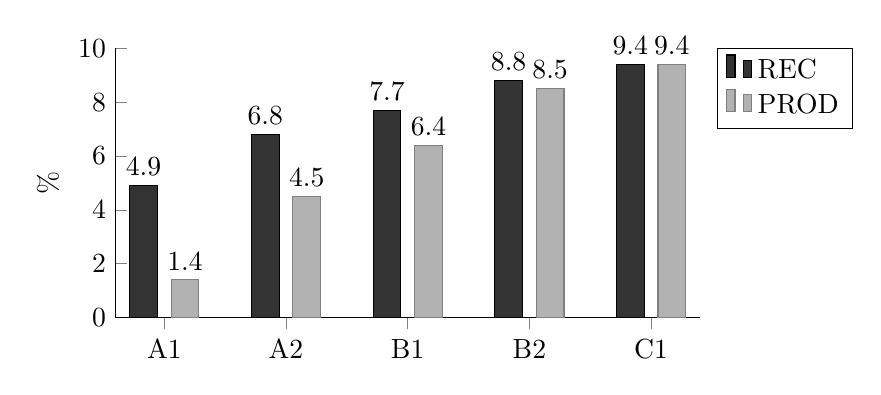
\begin{tikzpicture}
        \begin{axis}
            [ybar=5pt,
             ymin=0,
             ymax=10,
             ylabel=\%,
             ylabel near ticks,
             xtick=data,
             symbolic x coords={A1,A2,B1,B2,C1},
             bar width=1em,
             axis lines*=left,
             width=9cm,
             height=5cm,
             nodes near coords,
             nodes near coords style={black},
             legend pos=outer north east,
             legend cell align=left
            ]
            \addplot+ [draw=black, fill=black!80] coordinates
              {
                (A1,4.9) (A2,6.8) (B1,7.7) (B2,8.8) (C1,9.4)
              };
            \addlegendentry{REC}
            \addplot+ [draw=black!50, fill=black!30] coordinates
              {
                (A1,1.4) (A2,4.5) (B1,6.4) (B2,8.5) (C1,9.4) 
              };
            \addlegendentry{PROD}
        \end{axis}
    \end{tikzpicture}
    \caption{The percentage of MWEs on our sense-based list of lemgrams from Coctaill (REC) and SweLL-pilot (PROD)}
    \label{fig:MWElemgrams}
\end{figure}

The fact that data produced by L2 learners reach the same percentage of MWEs in the texts at C1 level as the percentage used in coursebooks at the same level seems very encouraging. It would be good to compare this with other corpora, but to do so in a reasonable way we would need to extract a list of types consisting of lemgram + sense in the same way as here and that will have to be left for future work. In addition, we should try to find a way to include MWEs which are partly non-normlike in the L2 data and which therefore have not been annotated by the pipeline, e.g. due to a mistaken form or non-normlike word order or even a word that is the wrong word in the context but synonymous. 
To study MWE acquisition we need to find ways to compare such occurrences to the rest; but, it seems they can only be captured manually unless they are consistent ‘mistakes’ which many learners tend to make.

\begin{figure} 
% % %     \includegraphics[width=12cm]{figures/09/con_non-con.png}
    \begin{tikzpicture}
	\pgfplotsset{
		% initialize Set1-5:
		cycle list/PuOr-4,
		% combine it with 'mark list*':
		cycle multiindex* list={
			mark list*\nextlist
			PuOr-4\nextlist
		},
	}
	\begin{axis}
		[smooth,
		 thick,
		 mark size=2.5pt,
		 ymin=0,
		 ymax=35,
		 xtick=data,
		 axis lines*=left,
		 symbolic x coords={A1,A2,B1,B2,C1},
		 width=9cm,
		 height=5cm,
		 legend pos=outer north east,
		 legend cell align=left
		]
		\addplot+ coordinates
		  {
		  	(A1,16.8291550603528) (A2,19.460317066822) (B1,18.8649796760381) (B2,24.2982564609868) (C1,23.1118011326547)
		  };
		\addlegendentry{Cont. Receptive}
		\addplot+ coordinates
		  {
		  	(A1,3.86697602474865) (A2,8.42367418693232) (B1,20.5206614895586) (B2,25.8296121180282) (C1,29.2038118659699) 
		  };
		\addlegendentry{Cont. Productive}
		\addplot+ coordinates
		  {
		    (A1,11.0259981429898) (A2,16.3615404638249) (B1,19.8150146237522) (B2,26.0294299493014) (C1,24.7584434525385) 
		  };
		\addlegendentry{Non-cont. Receptive}
		\addplot+ coordinates 
		  {
		    (A1,7.73395204949729) (A2,9.88866100205098) (B1,24.5443206051583) (B2,24.4200244200244) (C1,26.898247771288) 
		  };
		  \addlegendentry{Non-cont. Productive}
	\end{axis}
\end{tikzpicture}
    \caption{Development of contiguous and non-contiguous MWEs over CEFR proficiency levels in both coursebook data (receptive) and learner data (productive). The frequencies are based on the number of types in each category, not the frequency of occurrence of each type.}
    \label{fig:contiguity}
\end{figure}

Contiguous and non-contiguous MWEs show similar development over the CEFR levels as shown in Figure \ref{fig:contiguity}. There is a clear increase in both broad types of MWEs, and from B1 level contiguous MWEs have very similar levels in receptive and productive data. Surprisingly, there are more non-contiguous MWE lemmas in productive learner data from B1 than in the coursebook data. But from B2 the levels are similar in production too. The higher B1 level seems likely to be due to a task effect (cf. \citealt{caines2017effect}).  Of course we know that in the productive data we are only catching items which have been correctly spelled and might therefore miss some instances which are reasonably normlike and which are attempts to produce MWEs which learners are starting to grasp. It is also possible that some MWEs have been used in the wrong context or in an unidiomatic way. For instance, the preposition might be wrong, since prepositions are not usually included in the MWE in Saldo. This means that a non-standard preposition will not cause the MWE to go unnoticed by the system. This makes it even more interesting that at B1 level there were more non-contiguous MWE lemmas in the learner data than in coursebooks. Including less, in the MWE itself, proves to be a possible advantage when working with learner texts. If MWEs can be identified even when they are not used in a normlike manner, that facilitates a closer analysis of how normlike the usage is. 

Zooming in on the subcategories among the contiguous MWEs (Figures~\ref{fig:MWEcontig} \& \ref{fig:MWEcontig4b}), adverbial MWEs stand out at all levels in both the receptive and the productive data. It would be interesting to compare this to other genres. It is also striking that at A1, in the productive data, 
the only contiguous MWE type is contiguous adverbial MWEs, but at A2 there are already several others. The only subcategory among the contiguous MWEs which is still missing in the productive A2 data is proper nouns and this could possibly be related to pseudonymisation of the data, although it seems unlikely in this case since the MWE proper nouns that are included in Saldo are generally famous people, companies, organisations etc. This means that it is more likely to be the tasks at A2 that are restricting the use of MWE proper nouns. The category is still missing at B1 and is quite rare at B2 and very rare at C1.

\begin{figure}[p]
% %     \includegraphics[width=12cm]{figures/09/cont_recep.png}
    \pgfplotstableread{data/ch9-fig4.csv}\ChapterNineTableFour
    \begin{tikzpicture}
	\small
	\begin{axis}
		[
			ybar=1.5pt,
			ymin=0,
			ylabel near ticks,
			xticklabels from table={\ChapterNineTableFour}{Data},
			xtick=data,
			bar width=1ex,
			axis lines*=left,
			width=\textwidth,
			height=5cm,
			cycle list name=langsci-RdYlBu-5,
			x tick label style={text width=1.25cm, align=center,font=\sloppy}
		]
		\foreach \i in {A1,A2,B1,B2,C1}
		  {
		  	\addplot table [x expr=\coordindex, x=Data, y=\i] {\ChapterNineTableFour};
		    \edef\temp{\noexpand\addlegendentry{\i}}
		    \temp
 		  }
	\end{axis}
    \end{tikzpicture}
    \caption{Contiguous MWE types in coursebook data (receptive) over CEFR levels per 10 000 tokens, i.e. the frequency of occurrence (cf. tokens) of the different types (cf. lemmas) is not considered here.}
    \label{fig:MWEcontig}
\end{figure}

\begin{figure}[p]
% %     \includegraphics[width=12cm]{figures/09/cont_prod.png}
    \pgfplotstableread{data/ch9-fig5.csv}\ChapterNineTableFive
    \begin{tikzpicture}
	\small
	\begin{axis}
		[
			ybar=1.5pt,
			ymin=0,
			ylabel near ticks,
			xticklabels from table={\ChapterNineTableFive}{Data},
			xtick=data,
			bar width=1ex,
			axis lines*=left,
			width=\textwidth,
			height=5cm,
			cycle list name=langsci-RdYlBu-5,
			x tick label style={text width=1.25cm, align=center,font=\sloppy}
		]
		\foreach \i in {A1,A2,B1,B2,C1}
		  {
		  	\addplot table [x expr=\coordindex, x=Data, y=\i] {\ChapterNineTableFive};
		    \edef\temp{\noexpand\addlegendentry{\i}}
		    \temp
 		  }
	\end{axis}
    \end{tikzpicture}
    \caption{Contiguous MWE types in learner data (productive) over CEFR levels per 10 000 tokens, i.e. the frequency of occurrence (cf. tokens) of the different types (cf. lemmas) is not considered here.}
    \label{fig:MWEcontig4b}
\end{figure}

\begin{figure}[p]
% %     \includegraphics[width=12cm]{figures/09/non_cont.png}
    \newdimen\DimenTickLabelWidth
    \settowidth{\DimenTickLabelWidth}{prod.}
    \pgfplotstableread{data/ch9-fig6.csv}\ChapterNineTableSix
    \begin{tikzpicture}
	\small
	\begin{axis}
		[
			ybar=1.5pt,
			ymin=0,
			ylabel near ticks,
			xticklabels from table={\ChapterNineTableSix}{Data},
			xtick=data,
			bar width=1ex,
			axis lines*=left,
			width=\textwidth,
			height=5cm,
			enlarge y limits={value=0.25, upper},
			cycle list name=langsci-RdYlBu-5,
			x tick label style={text width=\DimenTickLabelWidth, align=center},
			legend pos=north west,
			legend cell align=left,
			legend columns=2
		]
		\foreach \i in {{Other verbal},{Support verb},{Particle verbs},{Reflexive verbs}}
		  {
		  	\addplot table [x expr=\coordindex, x=Data, y=\i] {\ChapterNineTableSix};
		    \edef\temp{\noexpand\addlegendentry{\i}}
		    \temp
 		  }
	\end{axis}
    \end{tikzpicture}
    \caption{Non-contiguous MWE types in relation to 10 000 tokens, i.e. the frequency of occurrence (tokens) of the different types (cf. lemmas) is not considered here.}
    \label{fig:MWEtypes10000}
\end{figure}

Interjections are quite rare in productive data and there is a decrease in the use of MWE interjections in the receptive data. Still, it is interesting that there are MWE interjections at all levels in the coursebooks, even at C1 level. It would be interesting to have a closer look at the interjections that appear and in which text types they are used in the coursebooks. One would expect that they would only be used in dialogues, but considering the fairly high number of lemmas at more advanced levels when dialogues are more rare this requires further analysis. The fact that they are rare in learner language is most likely due to the tasks.

All non-contiguous MWEs in our data are verbal (Figure \ref{fig:MWEtypes10000}). 
The most common subcategory by far is particle verbs in both receptive and productive data. The frequency clearly increases from A1 to B2 in the receptive data and then drops a bit at C1. In the productive data there is a drop at A2. Otherwise there is a steady increase, so it seems likely that the drop at A2 is task-related or a sign that they are starting to really produce MWEs which they know and not whole-phrase constructions. In the productive data there are no instances of the categories \textit{other} or \textit{reflexive verbs} at A1 and interestingly there are no support verb constructions at C1, this may well also be task related. 


Reflexive verbs start to appear at A2 in the learner data and show a clear increase at B1 and then remain quite stable. After this the levels are similar to the coursebook data possibly indicating that a ceiling has been reached. The number of lemmas are then slightly higher than in the coursebooks, but this is probably due to the topics covered in the respective texts. Reflexive verbs are quite common in different languages. However, the verbs which are reflexive differ even between closely related languages 
\citep[][41]{enstrom1990feltyper} (e.g. (sv) \textit{lära sig}
(lit. `teach oneself') ‘to learn’). In fact, they differ even between varieties of the same language, e.g. (sv) \textit{ändra sig}  
(lit. `change oneself') `change one’s mind' is not necessarily reflexive in Swedish as spoken in Finland \citep[cf.][]{af2008finlandssvensk}. \citet{bjorklund2007prep} similarly mentions differences in the usage of e.g. (sv) \textit{köpa sig}
(lit. `to buy oneself') `to buy' and (sv) \textit{köpa} `to buy' in Sweden and Finland, which however could be due to the small size of her data. 

It is quite possible that there may be interference from previously known languages which cause difficulty in learning which verbs are reflexive. It is likely that this is why it is quite common that the reflexive pronoun is left out. 
Furthermore, in relation to usage-based theories of language acquisition how easy it is to learn that a verb is reflexive or not could depend on which variety of the target language you have been in contact with more, if there is indeed variation with regards to whether the verb is reflexive in different varieties. Nevertheless, previous research has shown that there were not that many mistakes in connection with Swedish reflexive verbs, but they seemed to be underused both on the type and the token level in a comparison between L1 and advanced L2 writers \citep[][93–94]{enstrom1990feltyper}. 

The fact that \citet{enstrom1990feltyper} 
found that there were not many actual mistakes in comparison with the standard regarding how the reflexive verbs were used means that a quantitative comparison based on the reflexive MWEs is likely to give quite a correct image of the use in both coursebooks and learner texts. 
It is particularly interesting to see that the frequency of reflexive verbs at B1--C1 in our data is higher in the learner essays than in coursebooks. Quite possibly this is related to the essay topics, but it should be investigated further. 

\section{Conclusions and future work}\label{sec:Disc}

The Swedish L2 Profiles provides access to Swedish MWEs sorted by CEFR levels and with a possibility of comparing the usage in receptive and productive data by frequency as well as in context. This makes it a versatile resource e.g. for researchers and teachers, and it is clearly different from the English Profile and the Pearson Toolkit. Not only do MWEs occur in one place with a possibility to sort by types, but it also gives open access to frequencies and all of the empirical corpus evidence and presents \textit{productive} and \textit{receptive} overviews side by side. 

In this chapter we have summarised how 
we have ascertained that the know-ledge-based automatic MWE annotation works well enough for future studies of L2 Swedish. 
We have also presented our MWE taxonomy where we have tried to find an appropriate way of building on previous research and making it useful also in connection to automatic annotation.
The first round of manual annotation showed that some MWE types can be difficult to keep apart, but after adjusting our taxonomy the two annotators agreed quite well. 

Our attempts to find new ways of linking MWEs to receptive proficiency levels proved to work well only as relative measurements, not in relation to discrete levels \citep[][]{alfter2021mwe}. The best agreement seems to be with regards to ranking easy MWEs rather than difficult ones. This seems to have support in the CEFR documentation \citep{council2001common}, since the beginner levels have a very clear focus on certain topics and themes, whereas advanced levels are more varied because they relate to different areas of expertise \citep[cf.][]{lindstrom2022MWE}{}{}. 

In this chapter, we have extended our analysis of the crowdsourcing results through a qualitative analysis of items which were ranked differently than their coursebook first level of occurrence. 
The results indicate a possible tendency for items which occur in only one book at its first level of occurrence to be ranked less reliably based on coursebooks. This could be because we are investigating MWEs rather than single items, which previous work has focused on. Future research, should continue to investigate different ways of linking items to levels and make sure to investigate both single words and MWEs. If empirical data is used as a basis, rather than e.g. crowdsourcing, both receptive and productive data should be investigated.

Compositionality (or transparency)  
proved to be problematic since the annotators did not appear to have interpreted the task in the same way. Still, 
by using the compositionality score from \textit{one} of the annotators, we explore if there might be a tendency that relative rankings are linked to compositionality or transparency.   
Our results indicate that this might be the case, at least with regards to whether interjections or fixed expressions (group 1 in the crowdsourcing experiment) 
are interpreted as easier or more difficult than the first level of occurrence in coursebooks.  
This should be investigated further but it requires better ways of making sure whether it is transparency or compositionality that is estimated.

Some of the crowd rankings were also compared to occurrences in newspapers and blogs where the most difficult idiom was found to be rare in all of the corpora. Some further comparisons of this kind were done in a previous qualitative analysis \citep[][]{lindstrom2022MWE}{}{}, see also Section \ref{sec:easiest}. This showed that some MWEs may be more common in informal genres such as blogs, as claimed in \citet{prentice2013flerordsenheter}.

We see tendencies for MWE usage to depend on many different factors including the tasks and genres which we compare. This means that we need resources such as the Swedish L2 Profiles which facilitates the comparison of texts aimed at learners and texts written by learners, and which also provides a possibility of easily comparing data to other corpora.  
We also have to remember that learner data is often quite small and often consists of fairly short texts \citep[cf.][]{forsberg2010can}{}{} which can complicate analysis and in particular comparisons with L1 production which often consists of longer texts and much larger corpora.

Making use of the data from the Swedish L2 Profiles categorised into MWE types, we see 
a clear development for MWEs in both receptive and productive data. 
The percentage of MWEs among the lemgrams+sense types might possibly be an indicator of the productive proficiency level since there is a very clear increase per level and it is only at C1 that this is the same as in coursebooks at the group level, but also at B2 it is very close. Some subcategories show a clearer development (e.g. reflexive verbs, adverbial MWEs) whereas others seem fairly stable (e.g. support verbs, other contiguous MWEs such as idioms), and occasionally there is an indication of possible overuse.  
Future studies should try to investigate this further while restricting the genre and topic to match as much as possible, but also by investigating MWEs per text in both receptive and productive data in relation to the CEFR levels. However, this is complicated by the fact that learner texts tend to be rather short. This means that it is unlikely that several MWEs will be used in one text.

\section*{Acknowledgments}
We would like to thank Riksbankens Jubileumsfond who financed most of the work presented in this paper through grant P17-0716:1. Some parts were also financed by the University of Helsinki and by Språkbanken Text, the University of Gothenburg.

We also wish to thank the editors and the anonymous reviewers for their valuable feedback on earlier versions of this chapter.

\section*{Abbreviations}
\begin{tabularx}{\textwidth}{@{}lQ@{}}
CEFR & Common European Framework of Reference for Languages\\
GSE & Global Scale of English\\
L1 & first language\\
L2 & second language\\
MI & mutual information\\
MWE & multiword expression\\
NLP & natural language processing\\
NP & noun phrase\\
POS & part-of-speech\\
SAG & The Swedish Academy Grammar \citep[][]{teleman1999svenska}{}{}\\
SAOL & The Swedish Academy Glossary \citep[][]{akademien2015svenska}{}{}\\
\end{tabularx}


{\sloppy\printbibliography[heading=subbibliography,notkeyword=this]}

\end{document}
